% !TEX encoding = UTF-8 Unicode
% \documentclass{article}
% \usepackage{../../superstyle}
% \usepackage{listings}
% \usepackage{amsmath}
% \begin{document}
% remove all before

%oppgavetekst
Rerun the calculation as in Step 3 for the sinusoidal load. (Be sure to include the weight of the beam itself.) Set p = 100 kg/m and plot your computed solutions against the correct solution. Answer the questions from Step 3, and in addition the following one: Is the error at x = L proportional to $h^2$ as claimed above? You may want to plot the error versus h on a log–log graph to investigate this question. Does the condition number come into play?

\vspace{5mm}
Løsning

\begin{lstlisting}[caption={Oppgave5.m}]
feiltab = zeros(11,1); 
kondtab = zeros(11,1);
h = zeros(11,1);
minst = 100; 
minstTall = 100; 
for(eksp=1:11)
    n=10*(2.^eksp);
    h(eksp) = 2 / n;
    %tall1 = konstantkrefter2(n);
    tall1 = lagmatrise(n)\konstantkrefter2(n);
    tall2=korrektutregning2(n); 
    tall3 = tall1(n)-tall2(n); 
    if abs(tall3)<abs(minstTall)
        minst=n; 
        minstTall = tall3; 
    end
    feiltab(eksp)=abs(tall3);
    kondtab(eksp)=condest(lagmatrise(n));
end; 
disp(minst); 
display long; 
disp('Feilene er som folger:'); 
disp(feiltab);
disp('Kondisjonstallene:');
disp(kondtab);
% plot med logaritmiske akser, error vs h^2
loglog(h, h.^2, h, feiltab);
\end{lstlisting}

\begin{lstlisting}[caption={konstantkrefter2.m}]
function [B] = konstantkrefter2(n)
%legger inn rader fra oppgaveteksten. 
%lager høyresiden av matriseligningen. (h^4/EI) * f(x) 
%deler opp bjelken i n lengder med lengde h 
h = 2 / n;        
L=2;
p=100; 
g=-9.81; 
d=480; 
w=0.3;
t=0.03; 
p = 100;
%regner ut kraften f(x) 
kraft = d*w*t*g; 
%lager lengdevektor (langt ut på brettet) 
%definerer E og I som gitt i oppgaven
E = 1.3*10.^(10); 
I = (w*t.^3)/12; 
B = ones(n, 1);
for k=1:n
    xi=k*h; 
    B(k, 1)=g*d*w*t+(p*g*sin(xi*(pi/2)));
end;
B=B*h^4/(E*I);
\end{lstlisting}

\begin{lstlisting}[caption={korrektutregning2.m}]
function [riktig] = korrektutregning2(n)
%deler opp bjelken i n lengder med lengde h 
h = 2 / n;
%regner ut kraften f(x) 
kraft = -9.81*480*0.3*0.03;
%definerer E og I som gitt i oppgaven
E = 1.3*10.^(10); 
I = (0.3*0.03.^3)/12; 
L=2;
p=100; 
g=-9.81;
%initierer matrisen med høyde n
riktig = zeros(n, 1);
for k=1:n
    %hver x er lengden ut i planken vi befinner oss
    x = h * k;
    %formel fra boken, oppgitt i oppgave 4. 
    riktig(k,1)=kraft/(24*E*I)*x.^2*(x.^2-4*L*x+6*(L.^2))
    		+(p*g*L/(E*I*pi))*(L.^3/(pi.^3)*sin(pi/L*x)-(x.^3)/6+(L/2)*x.^2-L.^2/(pi.^2)*x);
end
\end{lstlisting}

\vspace{3mm}

\begin{figure}[h]
\centering
\begin{minipage}{.5\textwidth}
  \centering
  \includegraphics[width=0.5\textwidth]{sections/Exercise5/result5}
    % \includegraphics[width=0.5\textwidth]{result5}
    \caption{Errors - Exercise 5}
    \label{fig:result5}
\end{minipage}%
\begin{minipage}{.5\textwidth}
  \centering
  \includegraphics[width=0.6\textwidth]{sections/Exercise5/cond5}
    % \includegraphics[width=0.6\textwidth]{cond5}
    \caption{Condition numbers - Ex5}
    \label{fig:cond5}
\end{minipage}
\end{figure}

\begin{figure}[h!]
    \centering
    \includegraphics[width=1\textwidth]{sections/Exercise5/loglog5}
    % \includegraphics[width=1\textwidth]{loglog5}
    \caption{Loglog plot - Error(grønn) vs $h^2$}
    \label{fig:loglog5}
\end{figure}

% Answer the questions from Step 3, and in addition the following one: Is the error at x = L proportional to $h^2$ as claimed above? You may want to plot the error versus h on a log–log graph to investigate this question. Does the condition number come into play?

Feilene vises i figur \ref{fig:result5}, i motsetning til hvordan feilen økte med n i oppgave 3, så er den minste feilen her når n = 1280. Før dette vil feilen minke, men etterpå ser det ut som at kondisjonstallet har en større påvirkning, og feilen vil øke proporsjonalt med $h^2$ som man kan se i figur \ref{fig:loglog5}.

% Feilene vises i figur \ref{fig:errors3}, og man kan se at feilen øker når n øker, dette kan man se har en sterk sammenheng med kondisjonstallene som vist i figur \ref{fig:cond3}. Den minste feilen er når k = 1, altså når $n = 10\cdot2^1 = 20$.

% remove after
% \end{document}